\chapter{Especificación de requisitos}

\noindent\fbox{
	\parbox{\textwidth}{
		En esta sección se tratarán de recoger todos los detalles que definan y limiten el funcionamiento de la aplicación.
	}
}

\section{Personas: ¿Quienes lo podrían usar?}

Para poder hacernos una idea de los posibles usos del Asistente de Voz se ha decidido crear una serie de personas ficticias que, para poder facilitar algún aspecto de su vida, puedan usar este producto.

En las tablas de las siguientes páginas, podemos encontrar una información somera de estas personas:

\begin{itemize}
	\item \textbf{Irene Fernández}, una estudiante de Bachiller en una fase de exámenes finales antes de la Selectividad, donde acaba por planear su estudio y el tiempo que le queda para poder acabar el curso y entrar a su carrera vocacional en la Universidad.
	
	\item \textbf{Javier Pedrosa}, un funcionario que recientemente perdió parte de la visión por un accidente, entrando en una nueva fase de su vida donde la tecnología le ayuda a poder tener cierta autonomía.
\end{itemize}

Si bien estos casos pueden necesitar soluciones concretas, el objetivo con este proyecto es que si alguna función no se pudiera realizar en este momento, gracias a la modularidad cualquiera pudiera integrar alguna utilidad para suplir esas demandas.

\newpage

\begin{table}[H]
	\centering
	\begin{tabular}{|l|l|l|} 
		\hline
		Nombre       & Irene Fernández & \multirow{4}{*}{
			\begin{minipage}[t]{0.4\textwidth}
				\begin{center}
					 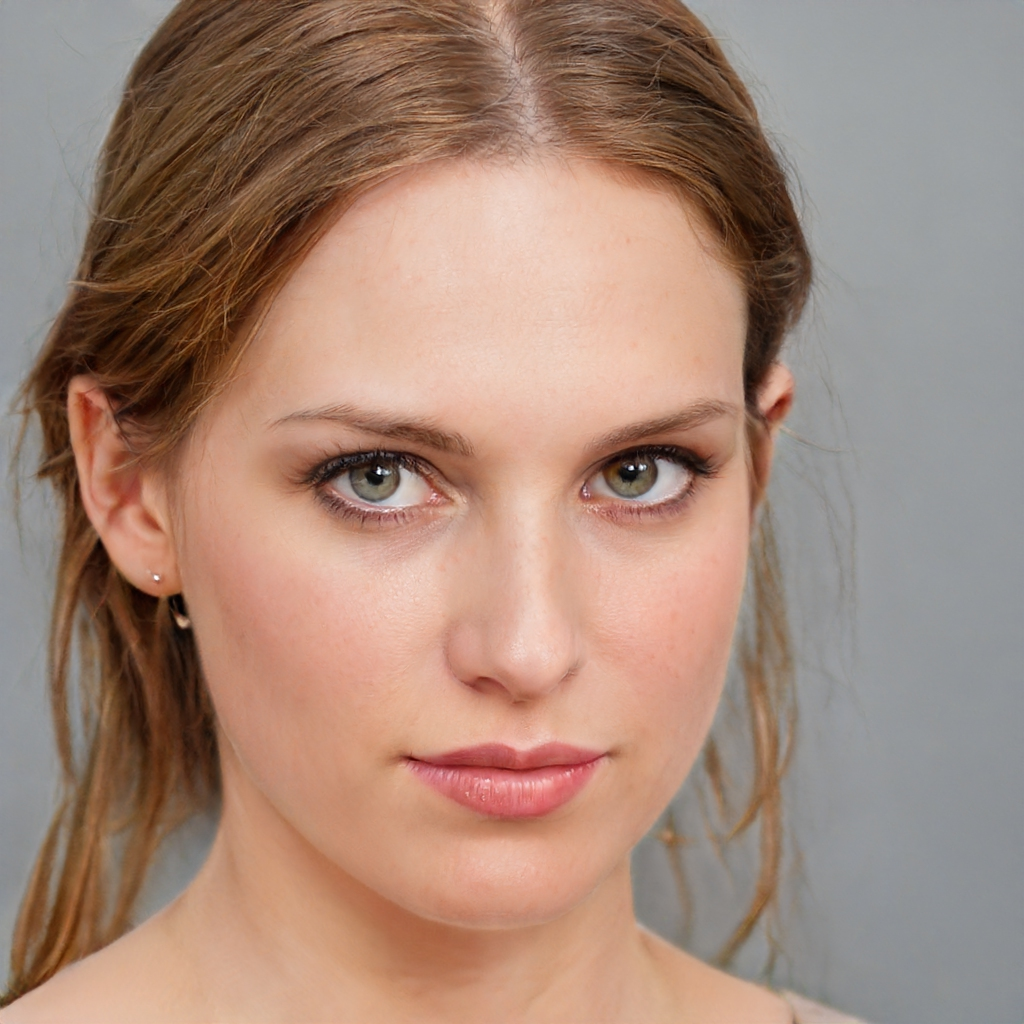
\includegraphics[height=3cm]{imagenes/Persona1.jpg}
				\end{center}
			\end{minipage}
			}                 \\ [2ex]
		\cline{1-2}
		Edad         & 19 &                                   \\ [2ex] 
		\cline{1-2}
		Género         & Femenino &                                   \\ [2ex]
		\cline{1-2}
		Educación    & Bachillerato Científico-Sanitario &                                   \\ [2ex] 
		\hline
		\multicolumn{3}{|l|}{\cellcolor{lightblue}\textbf{Contexto de uso}}               \\ 
		\hline
		Cuándo       & \multicolumn{2}{l|}{Tras las clases, antes de ponerse a estudiar}                \\ 
		\hline
		Dónde        & \multicolumn{2}{l|}{Ordenador portátil}                \\ 
		\hline
		\multicolumn{3}{|l|}{\cellcolor{lightblue}\textbf{Misión}}                        \\ 
		\hline
		Objetivo     & \multicolumn{2}{l|}{Tener una ayuda en el estudio}                \\ 
		\hline
		Expectativas & \multicolumn{2}{l|}{
			\begin{minipage} [t] {0.7\textwidth}
				\begin{itemize}
					\item Permitir hacer control del tiempo a través de contadores regresivos
					\item Permitir realizar cálculos sencillos
					\item Recordar tareas pendientes
				\end{itemize}
			\end{minipage}
		}                \\ 
		\hline
		\multicolumn{3}{|l|}{\cellcolor{lightblue}\textbf{Motivación}}                   \\ 
		\hline
		Urgencia     & \multicolumn{2}{l|}{
			\begin{minipage}[t]{0.7\textwidth}
				No le sería de mucha urgencia, ya que puede usar otras herramientas (Reloj/Cronómetro, Agenda, Calculadora...)
			\end{minipage}
		}                \\ 
		\hline
		Deseo        & \multicolumn{2}{l|}{
			\begin{minipage}[t]{0.7\textwidth}
				Siente que llevar tantas cosas para poder organizar su vida puede ser un tanto engorro, y centralizar sus utilidades en algo que lleve consigo como su portátil o su teléfono podría ahorrarle tantas molestias.
			\end{minipage}
		}                \\ 
		\hline
		\multicolumn{3}{|l|}{\cellcolor{lightblue}\textbf{Actitud ante la tecnología}}    \\ 
		\hline
		\multicolumn{3}{|l|}{
			\begin{minipage}[t]{\textwidth}
				Sabe manejar el ordenador en programas de ofimática como Word y Powerpoint; usa el navegador constantemente para ver sus redes sociales y buscar lo que necesite
			\end{minipage}
		}                              \\
		\hline
	\end{tabular}
	\caption[Ficha Persona 1]{Ficha de la Persona 1 (Irene Fernández). Imagen extraída de \cite{thispersondoesnotexist}}
\end{table}

\newpage

\begin{table}[H]
	\centering
	\begin{tabular}{|l|l|l|} 
		\hline
		Nombre       & Javier Pedrosa & \multirow{4}{*}{
			\begin{minipage}[t]{0.4\textwidth}
				\begin{center}
					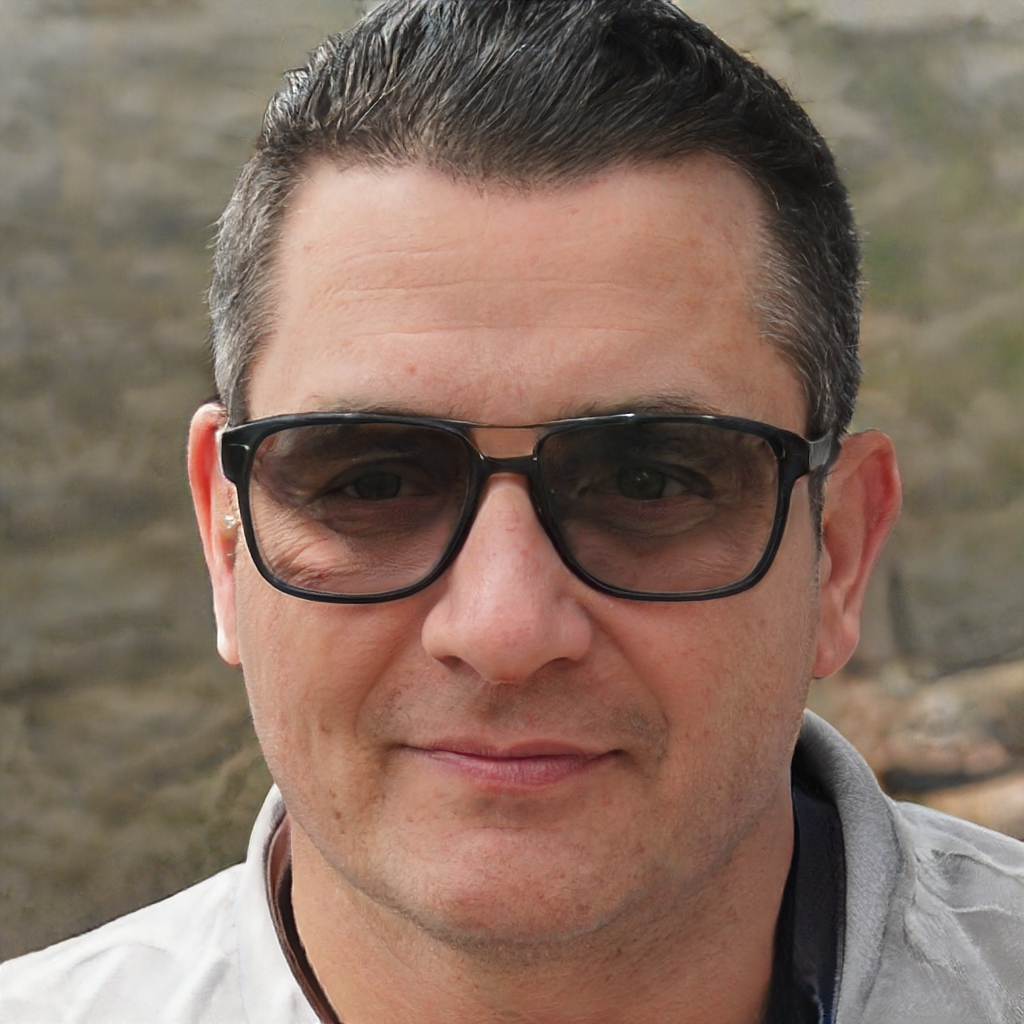
\includegraphics[height=3cm]{imagenes/Persona2.jpg}
				\end{center}
			\end{minipage}
		}                 \\ [2ex]
		\cline{1-2}
		Edad         & 46 &                                   \\ [2ex] 
		\cline{1-2}
		Género         & Masculino &                                   \\ [2ex]
		\cline{1-2}
		Profesión    & 
			\begin{minipage}[t]{0.3 \textwidth}
				Funcionario
			\end{minipage}
		 &                                   \\ [2ex] 
		\hline
		\multicolumn{3}{|l|}{\cellcolor{lightblue}\textbf{Contexto de uso}}               \\ 
		\hline
		Cuándo       & \multicolumn{2}{l|}{Al llegar a casa}                \\ 
		\hline
		Dónde        & \multicolumn{2}{l|}{Ordenador portátil y/o aparato dedicado}                \\ 
		\hline
		\multicolumn{3}{|l|}{\cellcolor{lightblue}\textbf{Misión}}                        \\ 
		\hline
		Objetivo     & \multicolumn{2}{l|}{Poder disfrutar de cierta independencia}                \\ 
		\hline
		Expectativas & \multicolumn{2}{l|}{
			\begin{minipage} [t] {0.7\textwidth}
				\begin{itemize}
					\item Permitir escuchar alguna información proveniente de Internet (Noticias, Tiempo...)
					\item Escuchar música, podcasts...
				\end{itemize}
			\end{minipage}
		}                \\ 
		\hline
		\multicolumn{3}{|l|}{\cellcolor{lightblue}\textbf{Motivación}}                   \\ 
		\hline
		Urgencia     & \multicolumn{2}{l|}{
			\begin{minipage}[t]{0.7\textwidth}
				No le sería de mucha urgencia, pero le encantaría tenerlo cuanto antes
			\end{minipage}
		}                \\ 
		\hline
		Deseo        & \multicolumn{2}{l|}{
			\begin{minipage}[t]{0.7\textwidth}
				Desde que perdió parcialmente la visión, no ha podido volver a dedicarse a pasiones como la literatura de forma fácil (por ejemplo, teniendo que esperar bastante tiempo para obtener audiolibros o libros adaptados a braille) o informarse en cualquier momento sin tener que pasar por el ordenador adaptado.
			\end{minipage}
		}                \\ 
		\hline
		\multicolumn{3}{|l|}{\cellcolor{lightblue}\textbf{Actitud ante la tecnología}}    \\ 
		\hline
		\multicolumn{3}{|l|}{
			\begin{minipage}[t]{\textwidth}
				Apenas usa el ordenador para alguna que otra gestión del trabajo.
			\end{minipage}
		}                              \\
		\hline
	\end{tabular}
	\caption[Ficha Persona 2]{Ficha de la Persona 2 (Javier Pedrosa). Imagen extraída de \cite{thispersondoesnotexist}}
\end{table}

\newpage

\section{Casos de uso: ¿Qué podrían hacer?}

Una vez pensado en posibles perfiles de uso, podríamos preguntarnos por alguna incidencia que pudiera solucionarse o facilitarse gracias al sistema resultante.

\subsection{Caso 1: Irene y el calendario de exámenes}

\subsection{Caso 2: Javier y las noticias}

\makebox{Con ello, cumplimos el Objetivo O-DD 1.}

\section{La Ingeniería de Requisitos en acción}

\subsection{Requisitos funcionales}

\begin{table}[H]
	\centering
	\begin{tabularx}{\textwidth}{|c|X|} 
		\hline
		\textbf{Nº de RF }          &  1 \\ 
		\hline
		\textbf{Nombre}         &  Hablar al Asistente \\ 
		\hline
		\textbf{Descripción}    &  Como usuario, quiero poder hablar con el programa para comunicarme con este \\ 
		\hline
		\textbf{Prioridad}      &  Alta  \\ 
		\hline
		\textbf{Entrada}        & Un sonido  \\ 
		\hline
		\textbf{Prerrequisitos} & Debe ser un audio hablado con la compresión que requiera las APIs que intervengan  \\ 
		\hline
		\textbf{Procesamiento}  &  Envía el audio para que el computador lo pueda entender \\ 
		\hline
		\textbf{Postcondición}  &  - \\
		\hline
	\end{tabularx}
	\caption{Descripción del Requisito Funcional 1: Hablar al Asistente}
\end{table}
\subsection{Requisitos no funcionales}